\documentclass[]{article}
\usepackage{lmodern}
\usepackage{amssymb,amsmath}
\usepackage{ifxetex,ifluatex}
\usepackage{fixltx2e} % provides \textsubscript
\ifnum 0\ifxetex 1\fi\ifluatex 1\fi=0 % if pdftex
  \usepackage[T1]{fontenc}
  \usepackage[utf8]{inputenc}
\else % if luatex or xelatex
  \ifxetex
    \usepackage{mathspec}
  \else
    \usepackage{fontspec}
  \fi
  \defaultfontfeatures{Ligatures=TeX,Scale=MatchLowercase}
\fi
% use upquote if available, for straight quotes in verbatim environments
\IfFileExists{upquote.sty}{\usepackage{upquote}}{}
% use microtype if available
\IfFileExists{microtype.sty}{%
\usepackage{microtype}
\UseMicrotypeSet[protrusion]{basicmath} % disable protrusion for tt fonts
}{}
\usepackage[margin=1in]{geometry}
\usepackage{hyperref}
\hypersetup{unicode=true,
            pdftitle={MATH1318 Time Series},
            pdfauthor={Phil Steinke s3725547},
            pdfborder={0 0 0},
            breaklinks=true}
\urlstyle{same}  % don't use monospace font for urls
\usepackage{color}
\usepackage{fancyvrb}
\newcommand{\VerbBar}{|}
\newcommand{\VERB}{\Verb[commandchars=\\\{\}]}
\DefineVerbatimEnvironment{Highlighting}{Verbatim}{commandchars=\\\{\}}
% Add ',fontsize=\small' for more characters per line
\usepackage{framed}
\definecolor{shadecolor}{RGB}{248,248,248}
\newenvironment{Shaded}{\begin{snugshade}}{\end{snugshade}}
\newcommand{\AlertTok}[1]{\textcolor[rgb]{0.94,0.16,0.16}{#1}}
\newcommand{\AnnotationTok}[1]{\textcolor[rgb]{0.56,0.35,0.01}{\textbf{\textit{#1}}}}
\newcommand{\AttributeTok}[1]{\textcolor[rgb]{0.77,0.63,0.00}{#1}}
\newcommand{\BaseNTok}[1]{\textcolor[rgb]{0.00,0.00,0.81}{#1}}
\newcommand{\BuiltInTok}[1]{#1}
\newcommand{\CharTok}[1]{\textcolor[rgb]{0.31,0.60,0.02}{#1}}
\newcommand{\CommentTok}[1]{\textcolor[rgb]{0.56,0.35,0.01}{\textit{#1}}}
\newcommand{\CommentVarTok}[1]{\textcolor[rgb]{0.56,0.35,0.01}{\textbf{\textit{#1}}}}
\newcommand{\ConstantTok}[1]{\textcolor[rgb]{0.00,0.00,0.00}{#1}}
\newcommand{\ControlFlowTok}[1]{\textcolor[rgb]{0.13,0.29,0.53}{\textbf{#1}}}
\newcommand{\DataTypeTok}[1]{\textcolor[rgb]{0.13,0.29,0.53}{#1}}
\newcommand{\DecValTok}[1]{\textcolor[rgb]{0.00,0.00,0.81}{#1}}
\newcommand{\DocumentationTok}[1]{\textcolor[rgb]{0.56,0.35,0.01}{\textbf{\textit{#1}}}}
\newcommand{\ErrorTok}[1]{\textcolor[rgb]{0.64,0.00,0.00}{\textbf{#1}}}
\newcommand{\ExtensionTok}[1]{#1}
\newcommand{\FloatTok}[1]{\textcolor[rgb]{0.00,0.00,0.81}{#1}}
\newcommand{\FunctionTok}[1]{\textcolor[rgb]{0.00,0.00,0.00}{#1}}
\newcommand{\ImportTok}[1]{#1}
\newcommand{\InformationTok}[1]{\textcolor[rgb]{0.56,0.35,0.01}{\textbf{\textit{#1}}}}
\newcommand{\KeywordTok}[1]{\textcolor[rgb]{0.13,0.29,0.53}{\textbf{#1}}}
\newcommand{\NormalTok}[1]{#1}
\newcommand{\OperatorTok}[1]{\textcolor[rgb]{0.81,0.36,0.00}{\textbf{#1}}}
\newcommand{\OtherTok}[1]{\textcolor[rgb]{0.56,0.35,0.01}{#1}}
\newcommand{\PreprocessorTok}[1]{\textcolor[rgb]{0.56,0.35,0.01}{\textit{#1}}}
\newcommand{\RegionMarkerTok}[1]{#1}
\newcommand{\SpecialCharTok}[1]{\textcolor[rgb]{0.00,0.00,0.00}{#1}}
\newcommand{\SpecialStringTok}[1]{\textcolor[rgb]{0.31,0.60,0.02}{#1}}
\newcommand{\StringTok}[1]{\textcolor[rgb]{0.31,0.60,0.02}{#1}}
\newcommand{\VariableTok}[1]{\textcolor[rgb]{0.00,0.00,0.00}{#1}}
\newcommand{\VerbatimStringTok}[1]{\textcolor[rgb]{0.31,0.60,0.02}{#1}}
\newcommand{\WarningTok}[1]{\textcolor[rgb]{0.56,0.35,0.01}{\textbf{\textit{#1}}}}
\usepackage{graphicx,grffile}
\makeatletter
\def\maxwidth{\ifdim\Gin@nat@width>\linewidth\linewidth\else\Gin@nat@width\fi}
\def\maxheight{\ifdim\Gin@nat@height>\textheight\textheight\else\Gin@nat@height\fi}
\makeatother
% Scale images if necessary, so that they will not overflow the page
% margins by default, and it is still possible to overwrite the defaults
% using explicit options in \includegraphics[width, height, ...]{}
\setkeys{Gin}{width=\maxwidth,height=\maxheight,keepaspectratio}
\IfFileExists{parskip.sty}{%
\usepackage{parskip}
}{% else
\setlength{\parindent}{0pt}
\setlength{\parskip}{6pt plus 2pt minus 1pt}
}
\setlength{\emergencystretch}{3em}  % prevent overfull lines
\providecommand{\tightlist}{%
  \setlength{\itemsep}{0pt}\setlength{\parskip}{0pt}}
\setcounter{secnumdepth}{0}
% Redefines (sub)paragraphs to behave more like sections
\ifx\paragraph\undefined\else
\let\oldparagraph\paragraph
\renewcommand{\paragraph}[1]{\oldparagraph{#1}\mbox{}}
\fi
\ifx\subparagraph\undefined\else
\let\oldsubparagraph\subparagraph
\renewcommand{\subparagraph}[1]{\oldsubparagraph{#1}\mbox{}}
\fi

%%% Use protect on footnotes to avoid problems with footnotes in titles
\let\rmarkdownfootnote\footnote%
\def\footnote{\protect\rmarkdownfootnote}

%%% Change title format to be more compact
\usepackage{titling}

% Create subtitle command for use in maketitle
\newcommand{\subtitle}[1]{
  \posttitle{
    \begin{center}\large#1\end{center}
    }
}

\setlength{\droptitle}{-2em}

  \title{MATH1318 Time Series}
    \pretitle{\vspace{\droptitle}\centering\huge}
  \posttitle{\par}
  \subtitle{Assignment 1 - Semester 1, 2019}
  \author{Phil Steinke s3725547}
    \preauthor{\centering\large\emph}
  \postauthor{\par}
    \date{}
    \predate{}\postdate{}
  

\begin{document}
\maketitle

\hypertarget{executive-summary}{%
\section{Executive Summary}\label{executive-summary}}

This report examines the decline of the thickness of Ozone layer over 90
years.

To find this, data was collected from 1927 to 2016 in Dobson units
(yearly changes). Where a negative value in the dataset represents a
decrease in Ozone thickness and a positive value represents an Ozone
increase in the thickness.

\hypertarget{goals}{%
\paragraph{Goals:}\label{goals}}

\begin{quote}
Your task is to analyse the data by using the analysis methods covered
in the first two modules of MATH1318 Time Series Analysis course in this
semester.
\end{quote}

\hypertarget{r-code-15}\label{r-code-15}}

\begin{Shaded}
\begin{Highlighting}[]
\NormalTok{packages <-}\StringTok{ }\KeywordTok{c}\NormalTok{(}\StringTok{'beepr'}\NormalTok{, }\StringTok{'RColorBrewer'}\NormalTok{, }\StringTok{'tidyr'}\NormalTok{, }\StringTok{'TSA'}\NormalTok{, }\StringTok{'TTR'}\NormalTok{, }\StringTok{'smooth'}\NormalTok{)}
\KeywordTok{InstallAndLoadPackages}\NormalTok{(packages, setLocalWorkingDirectory)}
\end{Highlighting}
\end{Shaded}

\begin{verbatim}
## [1] "# Check for installed packages, then install them"
\end{verbatim}

\begin{verbatim}
##        beepr RColorBrewer        tidyr          TSA          TTR 
##         TRUE         TRUE         TRUE         TRUE         TRUE 
##       smooth 
##         TRUE
\end{verbatim}

\begin{Shaded}
\begin{Highlighting}[]
\NormalTok{ozone <-}\StringTok{ }\KeywordTok{read.csv}\NormalTok{(}\StringTok{"raw-data/data1.csv"}\NormalTok{, }\DataTypeTok{header =} \OtherTok{FALSE}\NormalTok{)}
\NormalTok{ozone.ts <-}\StringTok{ }\KeywordTok{ts}\NormalTok{(}\KeywordTok{as.vector}\NormalTok{(ozone), }\DataTypeTok{start =} \DecValTok{1927}\NormalTok{, }\DataTypeTok{end =} \DecValTok{2016}\NormalTok{) }\CommentTok{# convert to timeseries}
\NormalTok{colourPallete <-}\StringTok{ }\KeywordTok{brewer.pal}\NormalTok{(}\DataTypeTok{n =} \DecValTok{10}\NormalTok{, }\DataTypeTok{name =} \StringTok{"BrBG"}\NormalTok{)}
\CommentTok{# display.brewer.pal(10, 'BrBG')}
\KeywordTok{cat}\NormalTok{(}\StringTok{"}\CharTok{\textbackslash{}014}\StringTok{"}\NormalTok{)}
\end{Highlighting}
\end{Shaded}



\begin{Shaded}
\begin{Highlighting}[]
\CommentTok{# ozone.ts %>% tail(n = 5)}
\NormalTok{ozone.ts }\OperatorTok\StringTok{ }\KeywordTok{dim}\NormalTok{()}
\end{Highlighting}
\end{Shaded}

\begin{verbatim}
## [1] 90  1
\end{verbatim}

\hypertarget{the-data}{%
\paragraph{The Data}\label{the-data}}

The ozone thickness series is given by \texttt{dataset1.csv} which
represents:

\begin{itemize}
\tightlist
\item
  thickness of Ozone layer 1927 to 2016 in Dobson units (yearly changes)
\item
  A negative value in the dataset represents a decrease in Ozone
  thickness
\item
  A positive value represents an Ozone increase in the thickness
\item
  The dataset is timeseries and includes 90 records
\end{itemize}

Data was obtained from our lecturer `Haydar Demirhan'. Given there is
only a single variable \texttt{thickness\ of\ Ozone\ layer}, and that
the ozone layer varies in thickness around the globe, this statistic
would either be from a single location, or an average around the globe.

\hypertarget{what-are-dobson-units}{%
\paragraph{What are Dobson units?}\label{what-are-dobson-units}}

\begin{quote}
The Dobson Unit is the most common unit for measuring ozone
concentration. Over the Earth's surface, the ozone layer's average
thickness is about 300 Dobson Units or a layer that is 3 millimeters
thick. - \url{https://ozonewatch.gsfc.nasa.gov/facts/dobson_SH.html}
\end{quote}

\hypertarget{initial-plot-declare}{%
\paragraph{Initial Plot Declare}\label{initial-plot-declare}}

\begin{Shaded}
\begin{Highlighting}[]
\NormalTok{t =}\StringTok{ }\KeywordTok{time}\NormalTok{(ozone.ts) }\CommentTok{# Create time points for model fitting}

\NormalTok{default_ylab =}\StringTok{ 'Ozone layer thickness (Dobson units)'}
\NormalTok{default_subtitle =}\StringTok{ 'thickness of Ozone layer 1927 to 2016 in Dobson units - yearly changes'}
\NormalTok{default_xlab =}\StringTok{ 'Year (1927-2016)'}

\NormalTok{doTimeSeriesPlot <-}\StringTok{ }\ControlFlowTok{function}\NormalTok{(}
\NormalTok{  x, }
  \DataTypeTok{xlab =}\NormalTok{ default_xlab,}
\NormalTok{  y,}
  \DataTypeTok{ylab =}\NormalTok{ default_ylab,}
\NormalTok{  lines,}
  \DataTypeTok{type =} \StringTok{'o'}\NormalTok{, }
  \DataTypeTok{title =} \StringTok{''}\NormalTok{,}
  \DataTypeTok{subtitle =}\NormalTok{ default_subtitle}
\NormalTok{  ) \{}
  \CommentTok{# par(bg = colourPallete[5]) # plot background}
  \KeywordTok{plot}\NormalTok{( }
\NormalTok{    x,}
\NormalTok{    y,}
    \DataTypeTok{col =}\NormalTok{ colourPallete[}\DecValTok{9}\NormalTok{],}
    \DataTypeTok{pch =} \DecValTok{19}\NormalTok{,}
    \DataTypeTok{type =}\NormalTok{ type,}
    \DataTypeTok{xlab =}\NormalTok{ xlab,}
    \DataTypeTok{ylab =}\NormalTok{ default_ylab)}
  \KeywordTok{title}\NormalTok{(}
    \DataTypeTok{main =}\NormalTok{ title,}
    \DataTypeTok{sub =}\NormalTok{ subtitle,}
    \DataTypeTok{col.main =}\NormalTok{ colourPallete[}\DecValTok{9}\NormalTok{],}
    \DataTypeTok{font.main =} \DecValTok{3}\NormalTok{)}
  \KeywordTok{points}\NormalTok{(x)}
  \ControlFlowTok{if}\NormalTok{(}\OperatorTok{!}\KeywordTok{missing}\NormalTok{(lines)) \{ lines \}}
\NormalTok{\}}
\end{Highlighting}
\end{Shaded}

\hypertarget{ozone-layer-thickness}{%
\paragraph{Ozone Layer Thickness}\label{ozone-layer-thickness}}

\begin{Shaded}
\begin{Highlighting}[]
\KeywordTok{doTimeSeriesPlot}\NormalTok{(}
  \DataTypeTok{x =}\NormalTok{ ozone.ts,}
  \DataTypeTok{y =} \OtherTok{NULL}\NormalTok{,}
  \DataTypeTok{title =} \StringTok{'Ozone layer thickness with simple moving average'}\NormalTok{,}
  \DataTypeTok{lines =} \KeywordTok{lines}\NormalTok{(}\KeywordTok{SMA}\NormalTok{(ozone.ts)))}
\end{Highlighting}
\end{Shaded}

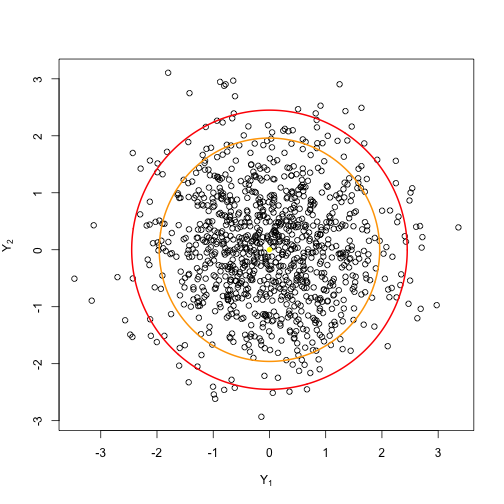
\includegraphics{assignment01-timeseries-psteinke_files/figure-latex/unnamed-chunk-3-1.pdf}

This plot shows:

\begin{itemize}
\tightlist
\item
  We can see a continuous decreasing trend
\item
  A negative slope
\item
  a decreasing simple moving average in thickness of ozone layer over 90
  years
\end{itemize}

\hypertarget{compare-data-with-its-previous-year}{%
\paragraph{Compare data with it's previous
year}\label{compare-data-with-its-previous-year}}

\begin{Shaded}
\begin{Highlighting}[]
\NormalTok{y =}\StringTok{ }\NormalTok{ozone.ts              }\CommentTok{# Read data into y}
\NormalTok{x =}\StringTok{ }\KeywordTok{zlag}\NormalTok{(ozone.ts)        }\CommentTok{# Generate first lag }
\NormalTok{index =}\StringTok{ }\DecValTok{2}\OperatorTok{:}\KeywordTok{length}\NormalTok{(x)          }\CommentTok{# Create an index to get rid of the first NA value and the last 5 missing values in x}
\KeywordTok{cor}\NormalTok{(y[index], x[index])}
\end{Highlighting}
\end{Shaded}

\begin{verbatim}
## [1] 0.8700381
\end{verbatim}

\begin{itemize}
\tightlist
\item
  A Correlation of 0.87 implies a strong positive relationship between
  the Ozone Layer thickness over time
\end{itemize}

\begin{Shaded}
\begin{Highlighting}[]
\KeywordTok{doTimeSeriesPlot}\NormalTok{(}
  \DataTypeTok{x =} \KeywordTok{zlag}\NormalTok{(ozone.ts), }\CommentTok{# Generate first lag of the series}
  \DataTypeTok{xlab =} \StringTok{'zlag'}\NormalTok{,}
  \DataTypeTok{y =}\NormalTok{ ozone.ts, }\CommentTok{# Read the data into y}
  \DataTypeTok{ylab =} \StringTok{'ozone.ts'}\NormalTok{,}
  \DataTypeTok{title =} \StringTok{"Compare ozone to previous/neighbouring year"}\NormalTok{,}
  \DataTypeTok{type=}\StringTok{'p'}\NormalTok{)}
\NormalTok{linearTrendModel_previousYear =}
\StringTok{  }\KeywordTok{lm}\NormalTok{(ozone.ts}\OperatorTok{~}\KeywordTok{zlag}\NormalTok{(ozone.ts))}
\KeywordTok{abline}\NormalTok{(}
\NormalTok{  linearTrendModel_previousYear,}
  \DataTypeTok{col =}\NormalTok{ colourPallete[}\DecValTok{1}\NormalTok{])}
\end{Highlighting}
\end{Shaded}

\includegraphics{assignment01-timeseries-psteinke_files/figure-latex/unnamed-chunk-5-1.pdf}
There is a strong positive autocorrolation of the data for concurrent
years.

\hypertarget{linear-trend}{%
\section{Linear Trend}\label{linear-trend}}

\hypertarget{model-1}{%
\subsection{Model 1}\label{model-1}}

\hypertarget{define-linear-trends-model}{%
\paragraph{Define Linear Trends
Model}\label{define-linear-trends-model}}

\begin{Shaded}
\begin{Highlighting}[]
\NormalTok{linearTrendModel =}\StringTok{ }\KeywordTok{lm}\NormalTok{(ozone.ts}\OperatorTok{~}\NormalTok{t)}
\end{Highlighting}
\end{Shaded}

\begin{Shaded}
\begin{Highlighting}[]
\KeywordTok{doTimeSeriesPlot}\NormalTok{(}
  \DataTypeTok{lines =} \KeywordTok{abline}\NormalTok{(}
\NormalTok{            linearTrendModel,}
            \DataTypeTok{col =}\NormalTok{ colourPallete[}\DecValTok{1}\NormalTok{]),}
  \DataTypeTok{title =} \StringTok{"Linear Trend of Ozone "}\NormalTok{,}
  \DataTypeTok{x =}\NormalTok{ ozone.ts,}
  \DataTypeTok{y =} \OtherTok{NULL}
\NormalTok{)}
\end{Highlighting}
\end{Shaded}

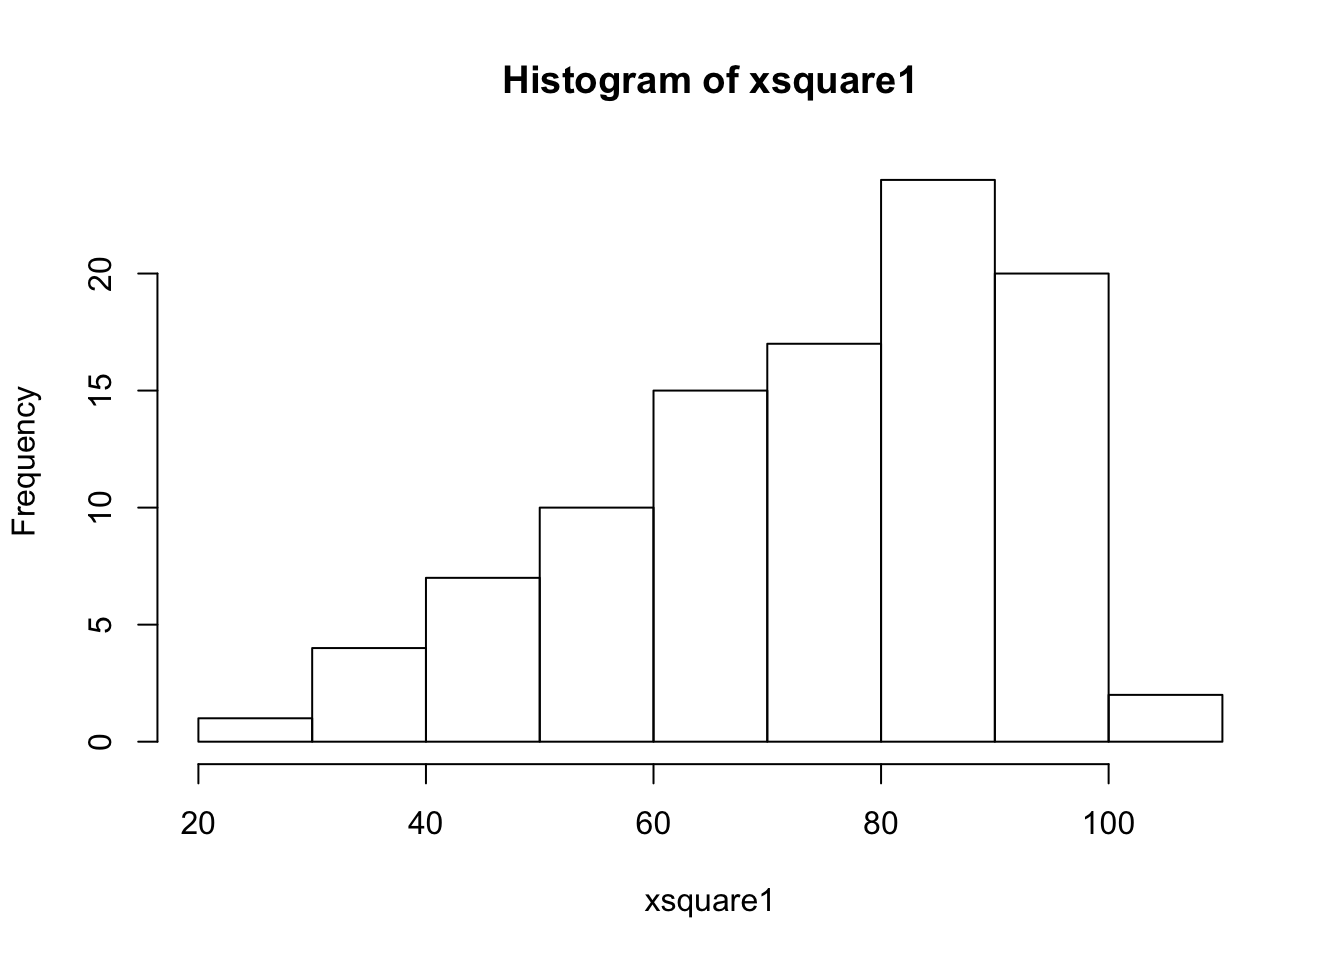
\includegraphics{assignment01-timeseries-psteinke_files/figure-latex/unnamed-chunk-7-1.pdf}
Initial visual inspection shows a linear trend does not continue to fit
the later years of the data

\hypertarget{linear-residuals}{%
\paragraph{Linear Residuals}\label{linear-residuals}}

\begin{Shaded}
\begin{Highlighting}[]
\NormalTok{t =}\StringTok{ }\KeywordTok{time}\NormalTok{(ozone.ts) }\CommentTok{# Create time points for model fitting}
\NormalTok{linearTrendModel =}\StringTok{ }\KeywordTok{lm}\NormalTok{(ozone.ts}\OperatorTok{~}\NormalTok{t) }\CommentTok{# label the model as model1}
\KeywordTok{summary}\NormalTok{(linearTrendModel)}
\end{Highlighting}
\end{Shaded}

\begin{verbatim}
## 
## Call:
## lm(formula = ozone.ts ~ t)
## 
## Residuals:
##     Min      1Q  Median      3Q     Max 
## -4.7165 -1.6687  0.0275  1.4726  4.7940 
## 
## Coefficients:
##               Estimate Std. Error t value Pr(>|t|)    
## (Intercept) 213.720155  16.257158   13.15   <2e-16 ***
## t            -0.110029   0.008245  -13.34   <2e-16 ***
## ---
## Signif. codes:  0 '***' 0.001 '**' 0.01 '*' 0.05 '.' 0.1 ' ' 1
## 
## Residual standard error: 2.032 on 88 degrees of freedom
## Multiple R-squared:  0.6693, Adjusted R-squared:  0.6655 
## F-statistic: 178.1 on 1 and 88 DF,  p-value: < 2.2e-16
\end{verbatim}

\begin{itemize}
\tightlist
\item
  a p-value \textless{} 0.05 shows that the model is significant
\item
  R2 = 0.6655 shows the model is partially significant
\end{itemize}

Slope: β̂1= -0.110029 Intercept: β̂̂00= 213.72015

\begin{Shaded}
\begin{Highlighting}[]
\NormalTok{res.linearTrendModel =}\StringTok{ }\KeywordTok{rstudent}\NormalTok{(linearTrendModel)}

\KeywordTok{doTimeSeriesPlot}\NormalTok{(}
  \DataTypeTok{x =} \KeywordTok{as.vector}\NormalTok{(}\KeywordTok{time}\NormalTok{(ozone.ts)),}
  \DataTypeTok{y =}\NormalTok{ res.linearTrendModel,}
  \DataTypeTok{title =} \StringTok{'Standardised Residuals of Linear Trends model '}\NormalTok{,}
  \DataTypeTok{subtitle =} \StringTok{'with Simple moving average'}\NormalTok{)}
\end{Highlighting}
\end{Shaded}

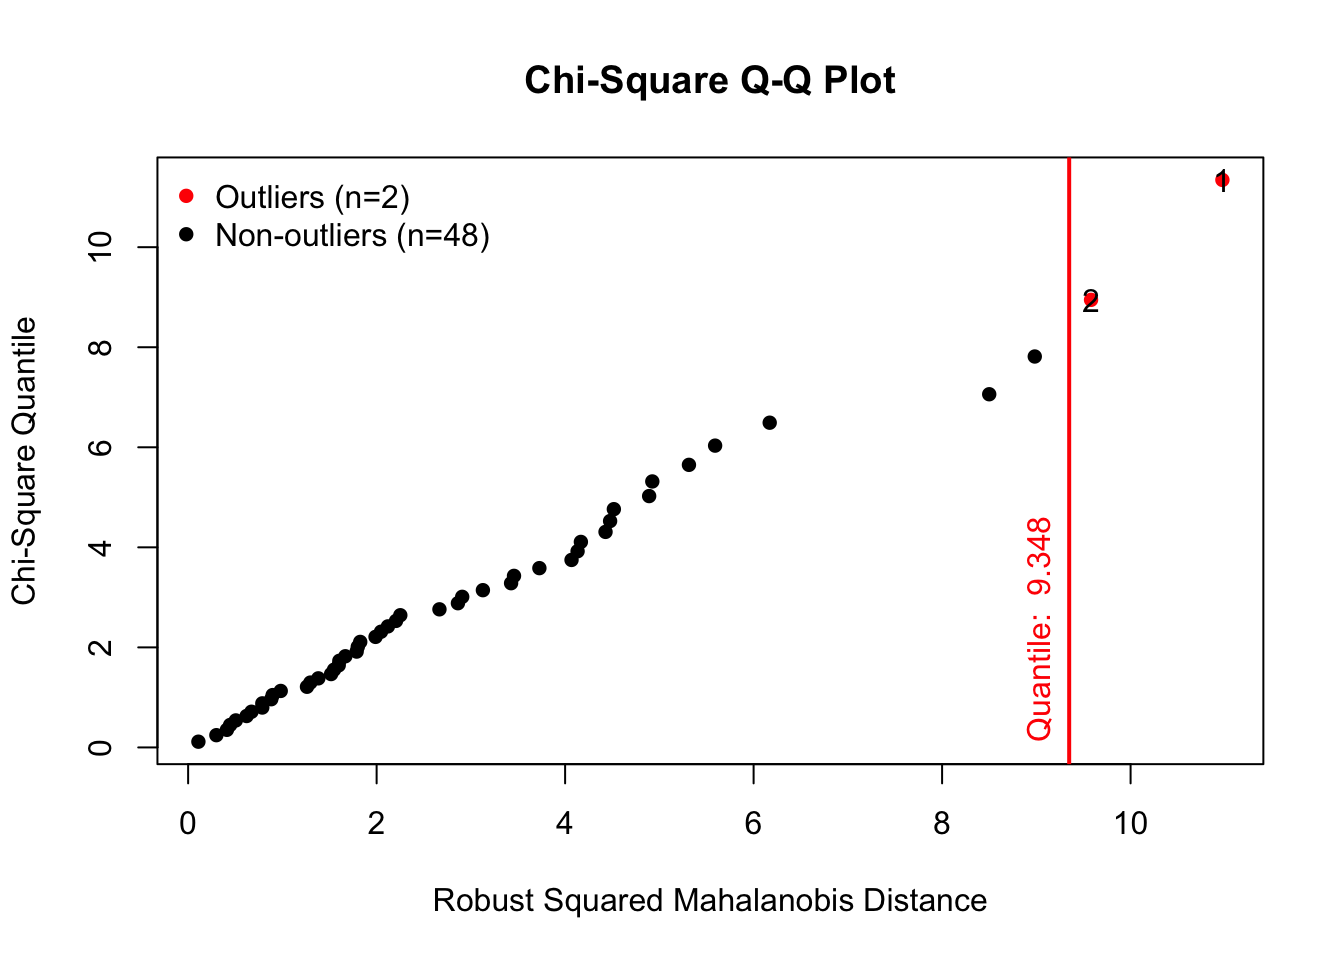
\includegraphics{assignment01-timeseries-psteinke_files/figure-latex/unnamed-chunk-9-1.pdf}

\begin{Shaded}
\begin{Highlighting}[]
\KeywordTok{qqnorm}\NormalTok{(res.linearTrendModel) }\CommentTok{# Q-Q Plot for normality}
\KeywordTok{abline}\NormalTok{(linearTrendModel)}
\KeywordTok{qqline}\NormalTok{(}
  \DataTypeTok{col =} \DecValTok{2}\NormalTok{,}
\NormalTok{  res.linearTrendModel,}
  \DataTypeTok{lty =} \DecValTok{2}\NormalTok{,}
  \DataTypeTok{lwd =} \DecValTok{1}\NormalTok{)}
\end{Highlighting}
\end{Shaded}

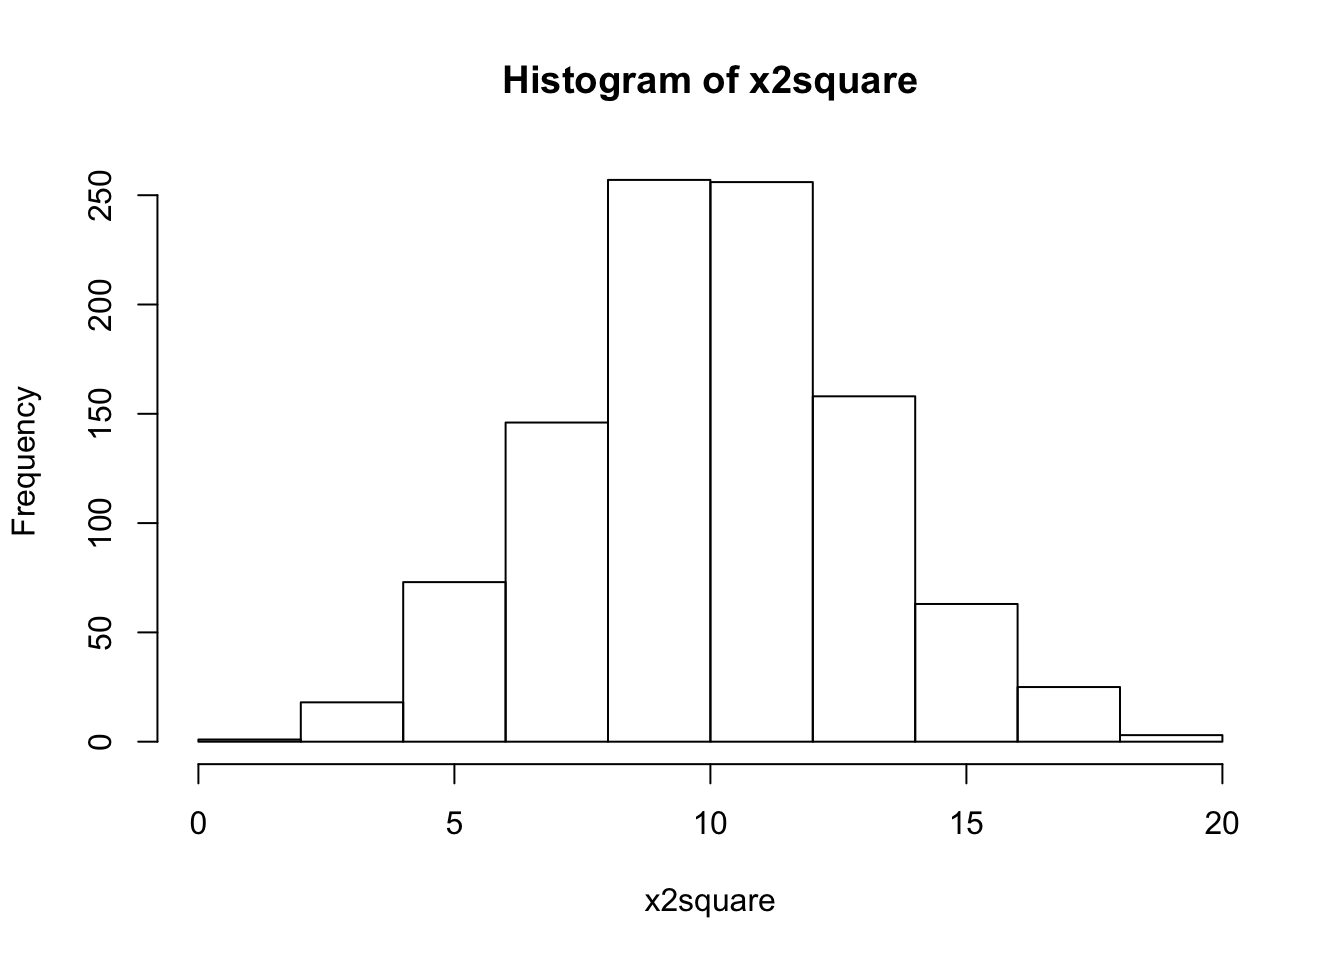
\includegraphics{assignment01-timeseries-psteinke_files/figure-latex/unnamed-chunk-10-1.pdf}

Q-Q plot shows significant skew indicating possible non-normality or
multi-modal data

\begin{Shaded}
\begin{Highlighting}[]
\KeywordTok{shapiro.test}\NormalTok{(res.linearTrendModel) }\CommentTok{# Check normality}
\end{Highlighting}
\end{Shaded}

\begin{verbatim}
## 
##  Shapiro-Wilk normality test
## 
## data:  res.linearTrendModel
## W = 0.98733, p-value = 0.5372
\end{verbatim}

\begin{Shaded}
\begin{Highlighting}[]
\KeywordTok{acf}\NormalTok{(res.linearTrendModel)}
\end{Highlighting}
\end{Shaded}

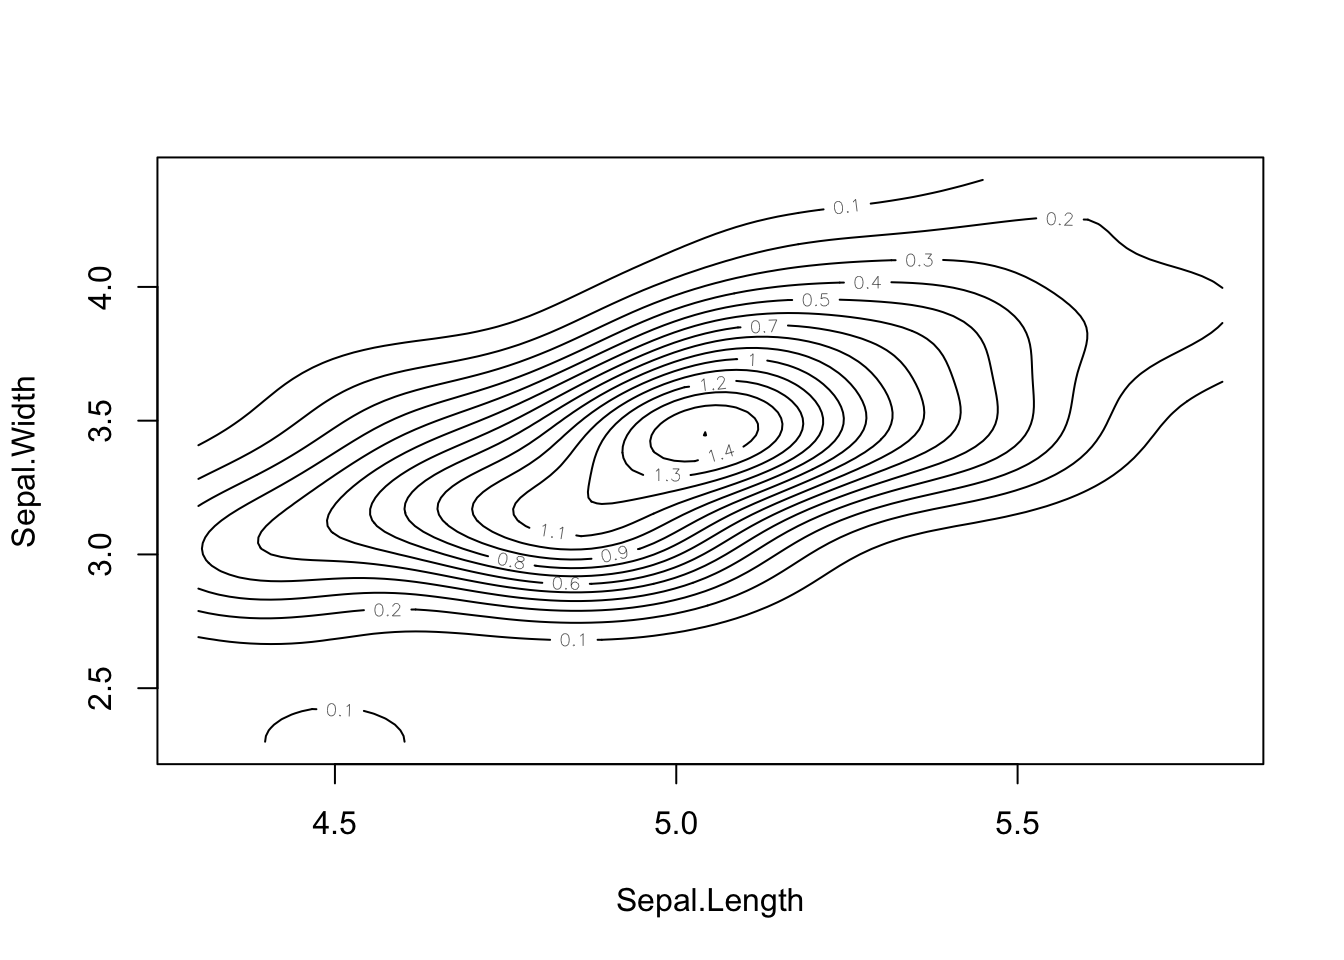
\includegraphics{assignment01-timeseries-psteinke_files/figure-latex/unnamed-chunk-12-1.pdf}

ACF shows that this data is not white noise. Shows outliers outside of
the 0.2 confidence region.

\hypertarget{forecast-for-linear}{%
\section{Forecast for Linear}\label{forecast-for-linear}}

\textbf{Task:} Give predictions of yearly changes for the next 5 years

\begin{Shaded}
\begin{Highlighting}[]
\NormalTok{doForecast <-}\StringTok{ }\ControlFlowTok{function}\NormalTok{(ourModel, start, plotTitle, ...) \{}
\NormalTok{  args <-}\StringTok{ }\KeywordTok{list}\NormalTok{(...)}
\NormalTok{  exist <-}\StringTok{ "t2"} \OperatorTok\StringTok{ }\KeywordTok{names}\NormalTok{(args)}
  
\NormalTok{  t =}\StringTok{ }\KeywordTok{c}\NormalTok{(}\DecValTok{2017}\OperatorTok{:}\DecValTok{2021}\NormalTok{)}
\NormalTok{  t2 =}\StringTok{ }\NormalTok{t }\OperatorTok{^}\StringTok{ }\DecValTok{2}

  \ControlFlowTok{if}\NormalTok{(exist) \{ new =}\StringTok{ }\KeywordTok{data.frame}\NormalTok{(t, t2) \} }
  \ControlFlowTok{else}\NormalTok{ \{ new =}\StringTok{ }\KeywordTok{data.frame}\NormalTok{(t) \}}
  
  \CommentTok{# Two-step algorithm}
\NormalTok{  forecasts =}\StringTok{ }\KeywordTok{predict}\NormalTok{(ourModel, new, }\DataTypeTok{interval =} \StringTok{"prediction"}\NormalTok{)}
  \KeywordTok{print}\NormalTok{(forecasts) }\CommentTok{# predicted interval}

  \KeywordTok{plot}\NormalTok{(}
\NormalTok{    ozone.ts, }
    \DataTypeTok{xlim =} \KeywordTok{c}\NormalTok{(}\DecValTok{1940}\NormalTok{,}\DecValTok{2022}\NormalTok{),}
    \DataTypeTok{ylim =} \KeywordTok{c}\NormalTok{(}\OperatorTok{-}\DecValTok{15}\NormalTok{,}\DecValTok{3}\NormalTok{),}
    \DataTypeTok{ylab =} \StringTok{""}\NormalTok{)}
  \KeywordTok{lines}\NormalTok{(}\KeywordTok{ts}\NormalTok{(}\KeywordTok{as.vector}\NormalTok{(forecasts[,}\DecValTok{1}\NormalTok{]), start), }\DataTypeTok{col=}\StringTok{"red"}\NormalTok{, }\DataTypeTok{type=}\StringTok{"l"}\NormalTok{)}
  \KeywordTok{lines}\NormalTok{(}\KeywordTok{ts}\NormalTok{(}\KeywordTok{as.vector}\NormalTok{(forecasts[,}\DecValTok{2}\NormalTok{]), start), }\DataTypeTok{col=}\StringTok{"blue"}\NormalTok{, }\DataTypeTok{type=}\StringTok{"l"}\NormalTok{)}
  \KeywordTok{lines}\NormalTok{(}\KeywordTok{ts}\NormalTok{(}\KeywordTok{as.vector}\NormalTok{(forecasts[,}\DecValTok{3}\NormalTok{]), start), }\DataTypeTok{col=}\StringTok{"blue"}\NormalTok{, }\DataTypeTok{type=}\StringTok{"l"}\NormalTok{)}
  \KeywordTok{legend}\NormalTok{(}
    \StringTok{"bottomleft"}\NormalTok{,}
    \KeywordTok{c}\NormalTok{(}\StringTok{"Data"}\NormalTok{,}\StringTok{"5% forecast limits"}\NormalTok{, }\StringTok{"Forecasts"}\NormalTok{),}
    \DataTypeTok{col=}\KeywordTok{c}\NormalTok{(}\StringTok{"black"}\NormalTok{,}\StringTok{"blue"}\NormalTok{,}\StringTok{"red"}\NormalTok{), }
    \DataTypeTok{lty=}\DecValTok{1}\NormalTok{, }
    \DataTypeTok{pch=}\DecValTok{1}\NormalTok{, }
    \DataTypeTok{text.width =} \DecValTok{20}\NormalTok{)}
    \KeywordTok{title}\NormalTok{(}
    \DataTypeTok{main =}\NormalTok{ plotTitle,}
    \DataTypeTok{sub =} \StringTok{'thickness of Ozone layer 1927 to 2016 in Dobson units - yearly changes'}\NormalTok{,}
    \DataTypeTok{col.main =}\NormalTok{ colourPallete[}\DecValTok{9}\NormalTok{],}
    \DataTypeTok{font.main =} \DecValTok{3}\NormalTok{)}
\NormalTok{\}}
\end{Highlighting}
\end{Shaded}

\begin{Shaded}
\begin{Highlighting}[]
\KeywordTok{doForecast}\NormalTok{(linearTrendModel, }\DecValTok{2016}\NormalTok{, }\StringTok{'Linear Trend Model'}\NormalTok{)}
\end{Highlighting}
\end{Shaded}

\begin{verbatim}
##         fit       lwr       upr
## 1 -8.208590 -12.33732 -4.079864
## 2 -8.318619 -12.45033 -4.186902
## 3 -8.428648 -12.56342 -4.293878
## 4 -8.538677 -12.67656 -4.400792
## 5 -8.648706 -12.78977 -4.507643
\end{verbatim}

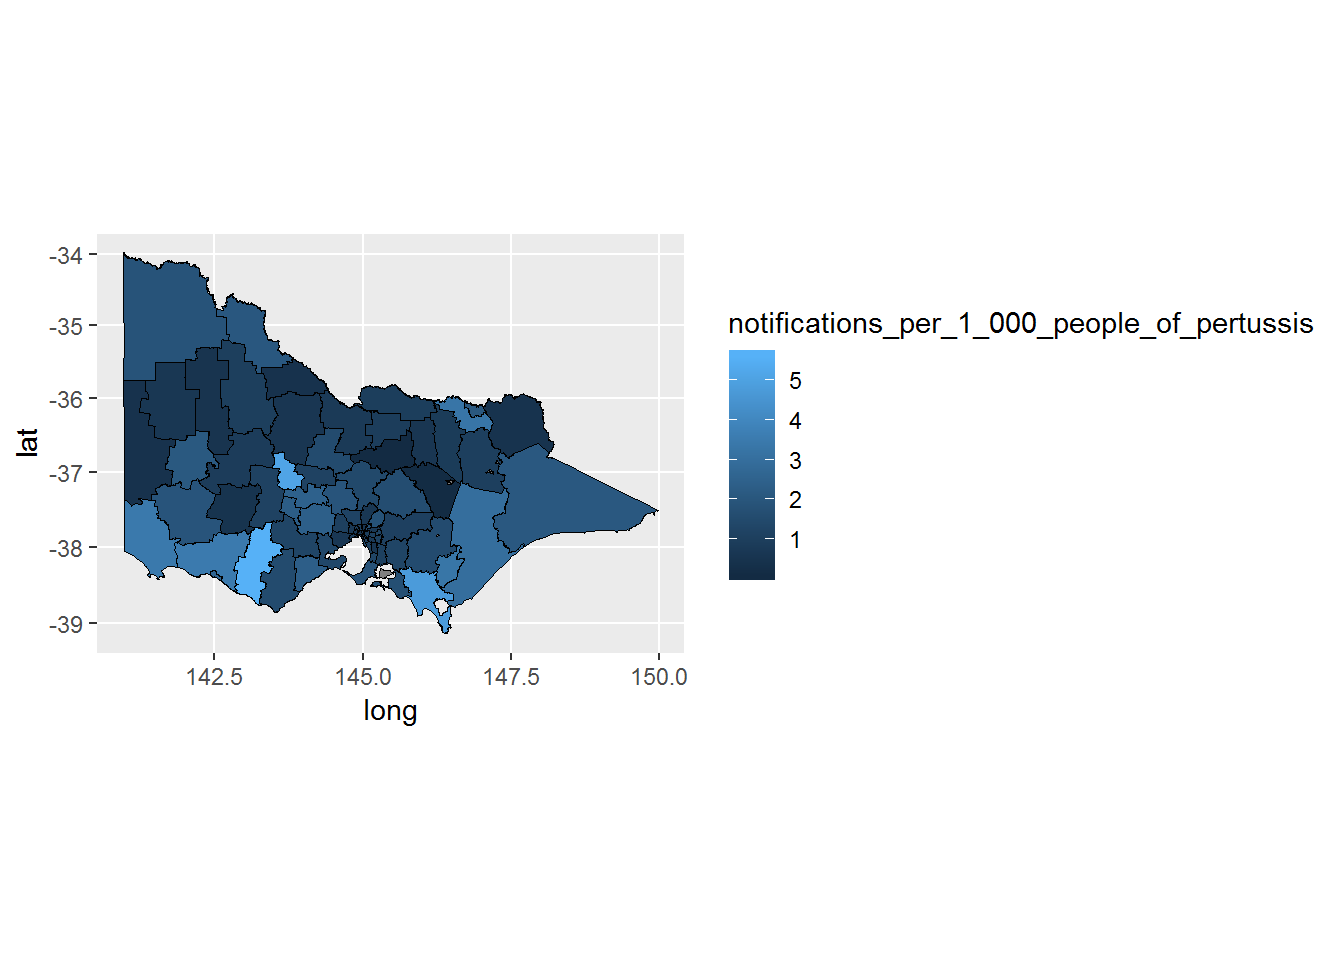
\includegraphics{assignment01-timeseries-psteinke_files/figure-latex/unnamed-chunk-14-1.pdf}

\hypertarget{hypothesis-for-linear}{%
\paragraph{Hypothesis for Linear}\label{hypothesis-for-linear}}

H0:μΔ=0 HA:μΔ≠0 reject hypothesis because data is not normal The
stochastic component of model 2 is not normally distributed

H0: yt ≠ β0 + β1xt + εt Ha: yt = β0 + β1xt + εt

We found that as the p-value was less than 5\% and the null mean
(i.e.~zero) fell within the 95\% confidence interval. As such the null
hypothesis was rejected.

\hypertarget{quadratic-time-trends}{%
\section{Quadratic time trends}\label{quadratic-time-trends}}

\hypertarget{model-2}{%
\subsection{Model 2}\label{model-2}}

\begin{itemize}
\tightlist
\item
  Use the least squares approach to fit a quadratic time trend to the
  Ozone data
\end{itemize}

\begin{Shaded}
\begin{Highlighting}[]
\CommentTok{# t = time(ozone.ts)}
\NormalTok{t2 =}\StringTok{ }\NormalTok{t}\OperatorTok{^}\DecValTok{2} \CommentTok{# square it}
\NormalTok{model.ozone.qa =}\StringTok{ }
\StringTok{  }\KeywordTok{lm}\NormalTok{(ozone.ts }\OperatorTok{~}\StringTok{ }\NormalTok{t }\OperatorTok{+}\StringTok{ }\NormalTok{t2) }\CommentTok{# label the quadratic trend model}
\KeywordTok{summary}\NormalTok{(model.ozone.qa)}
\end{Highlighting}
\end{Shaded}

\begin{verbatim}
## 
## Call:
## lm(formula = ozone.ts ~ t + t2)
## 
## Residuals:
##     Min      1Q  Median      3Q     Max 
## -5.1062 -1.2846 -0.0055  1.3379  4.2325 
## 
## Coefficients:
##               Estimate Std. Error t value Pr(>|t|)    
## (Intercept) -5.733e+03  1.232e+03  -4.654 1.16e-05 ***
## t            5.924e+00  1.250e+00   4.739 8.30e-06 ***
## t2          -1.530e-03  3.170e-04  -4.827 5.87e-06 ***
## ---
## Signif. codes:  0 '***' 0.001 '**' 0.01 '*' 0.05 '.' 0.1 ' ' 1
## 
## Residual standard error: 1.815 on 87 degrees of freedom
## Multiple R-squared:  0.7391, Adjusted R-squared:  0.7331 
## F-statistic: 123.3 on 2 and 87 DF,  p-value: < 2.2e-16
\end{verbatim}

\textbf{p:} 2.2e-16 \textless{} 0.05 \textbf{F:} 87 DF \textbf{R2:}
0.7331 shows the model is more significant than our linear model

\begin{Shaded}
\begin{Highlighting}[]
\KeywordTok{plot}\NormalTok{(}
  \KeywordTok{ts}\NormalTok{(}\KeywordTok{fitted}\NormalTok{(model.ozone.qa)),}
  \DataTypeTok{ylab =}\NormalTok{ default_ylab,}
  \DataTypeTok{ylim =} \KeywordTok{c}\NormalTok{(}
    \KeywordTok{min}\NormalTok{(}\KeywordTok{c}\NormalTok{(}
      \KeywordTok{fitted}\NormalTok{(model.ozone.qa),}
      \KeywordTok{as.vector}\NormalTok{(ozone.ts)}
\NormalTok{    )),}
    \KeywordTok{max}\NormalTok{(}\KeywordTok{c}\NormalTok{(}
      \KeywordTok{fitted}\NormalTok{(model.ozone.qa),}
      \KeywordTok{as.vector}\NormalTok{(ozone.ts)}
\NormalTok{    ))}
\NormalTok{  ),}
  \DataTypeTok{col =} \StringTok{"red"}\NormalTok{,}
  \DataTypeTok{lty =} \DecValTok{2}\NormalTok{,}
  \DataTypeTok{main =} \StringTok{"Fitted quadratic curve to ozone data"}\NormalTok{,}
  \DataTypeTok{type =} \StringTok{"l"}\NormalTok{,}
  \DataTypeTok{lines =} \KeywordTok{lines}\NormalTok{(}\KeywordTok{as.vector}\NormalTok{(ozone.ts), }\DataTypeTok{type =} \StringTok{"o"}\NormalTok{)}
\NormalTok{  )}
\KeywordTok{lines}\NormalTok{(}\KeywordTok{as.vector}\NormalTok{(ozone.ts), }\DataTypeTok{type =} \StringTok{"o"}\NormalTok{)}
\end{Highlighting}
\end{Shaded}

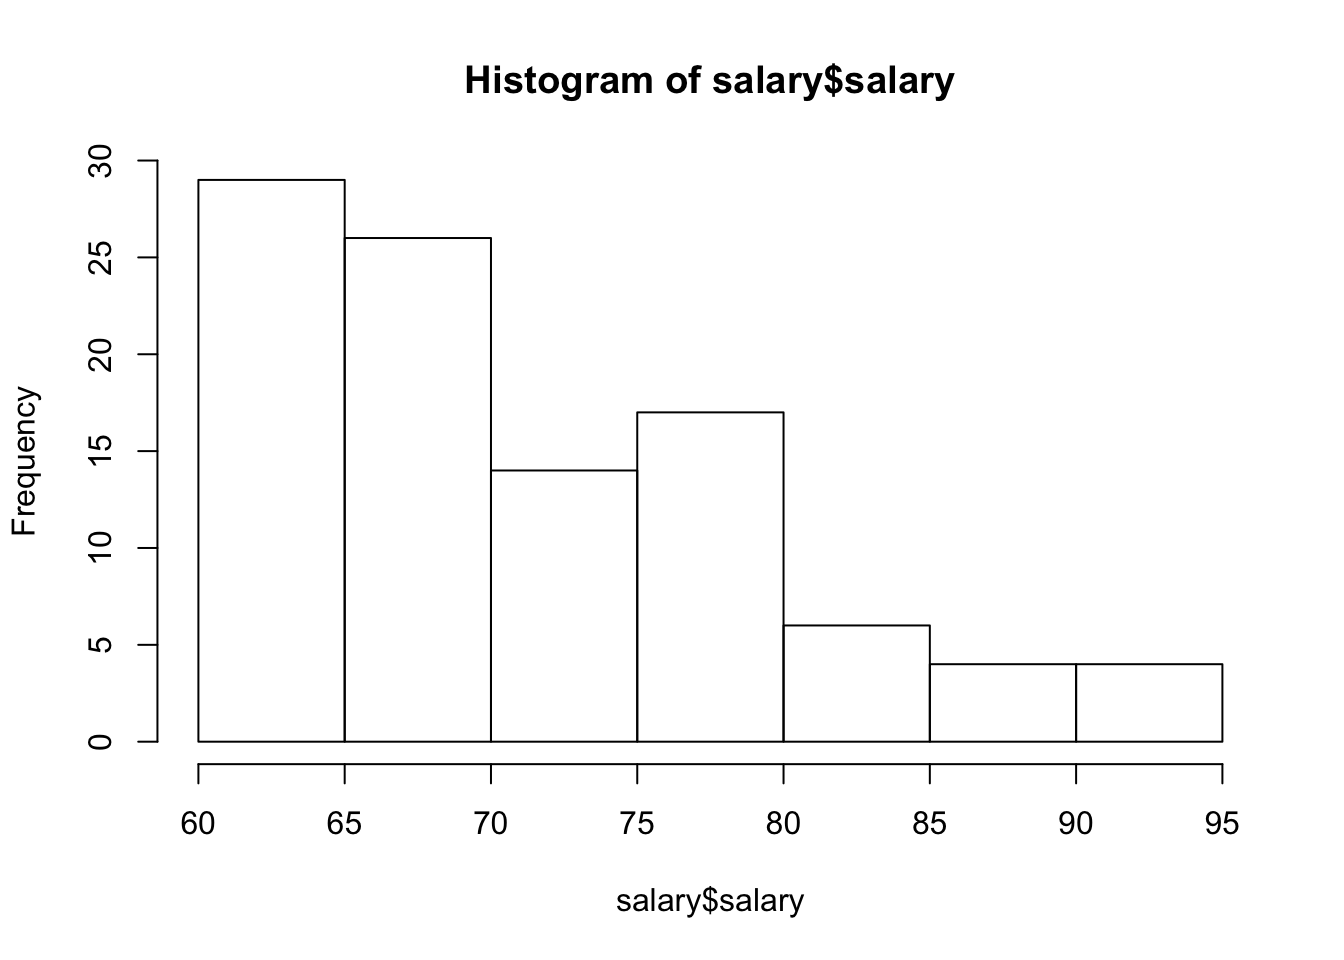
\includegraphics{assignment01-timeseries-psteinke_files/figure-latex/unnamed-chunk-15-1.pdf}

Visual inspection shows a closer fit to the data than linear

\hypertarget{quadratic-residuals}{%
\paragraph{Quadratic residuals}\label{quadratic-residuals}}

\begin{Shaded}
\begin{Highlighting}[]
\NormalTok{res.model.ozone.qa =}\StringTok{ }\KeywordTok{rstudent}\NormalTok{(model.ozone.qa)}
\KeywordTok{plot}\NormalTok{(}
  \DataTypeTok{x =} \KeywordTok{as.vector}\NormalTok{(}\KeywordTok{time}\NormalTok{(ozone.ts)),}
  \DataTypeTok{xlab =} \StringTok{'Years'}\NormalTok{,}
  \DataTypeTok{ylab =} \StringTok{'Standardized Residuals'}\NormalTok{,}
  \DataTypeTok{y =}\NormalTok{ res.model.ozone.qa,}
  \DataTypeTok{type =} \StringTok{'o'}\NormalTok{)}
\end{Highlighting}
\end{Shaded}

\includegraphics{assignment01-timeseries-psteinke_files/figure-latex/unnamed-chunk-16-1.pdf}

Standardised residual shows a moving average

\begin{Shaded}
\begin{Highlighting}[]
\KeywordTok{qqnorm}\NormalTok{(res.model.ozone.qa) }\CommentTok{# Q-Q Plot for normality}
\KeywordTok{qqline}\NormalTok{(}
\NormalTok{  res.model.ozone.qa,}
  \DataTypeTok{col =} \DecValTok{2}\NormalTok{,}
  \DataTypeTok{lty =} \DecValTok{2}\NormalTok{,}
  \DataTypeTok{lwd =} \DecValTok{1}\NormalTok{)}
\end{Highlighting}
\end{Shaded}

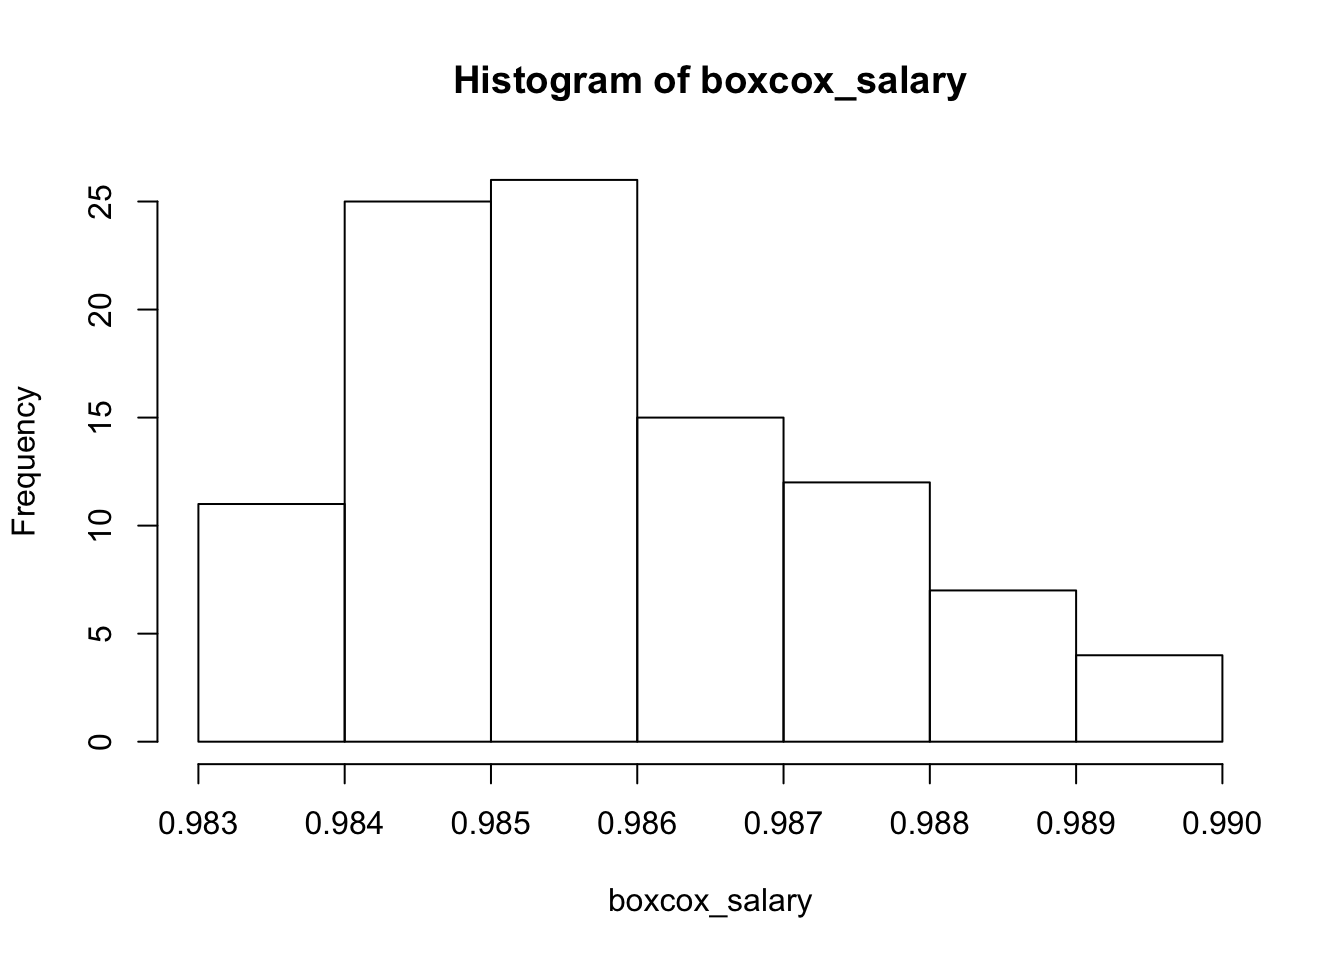
\includegraphics{assignment01-timeseries-psteinke_files/figure-latex/unnamed-chunk-17-1.pdf}

Data is not normal because Q-Q plot has some skew towards the final
data. However, it is less skewed than the linear model

\begin{Shaded}
\begin{Highlighting}[]
\KeywordTok{acf}\NormalTok{(res.model.ozone.qa)}
\end{Highlighting}
\end{Shaded}

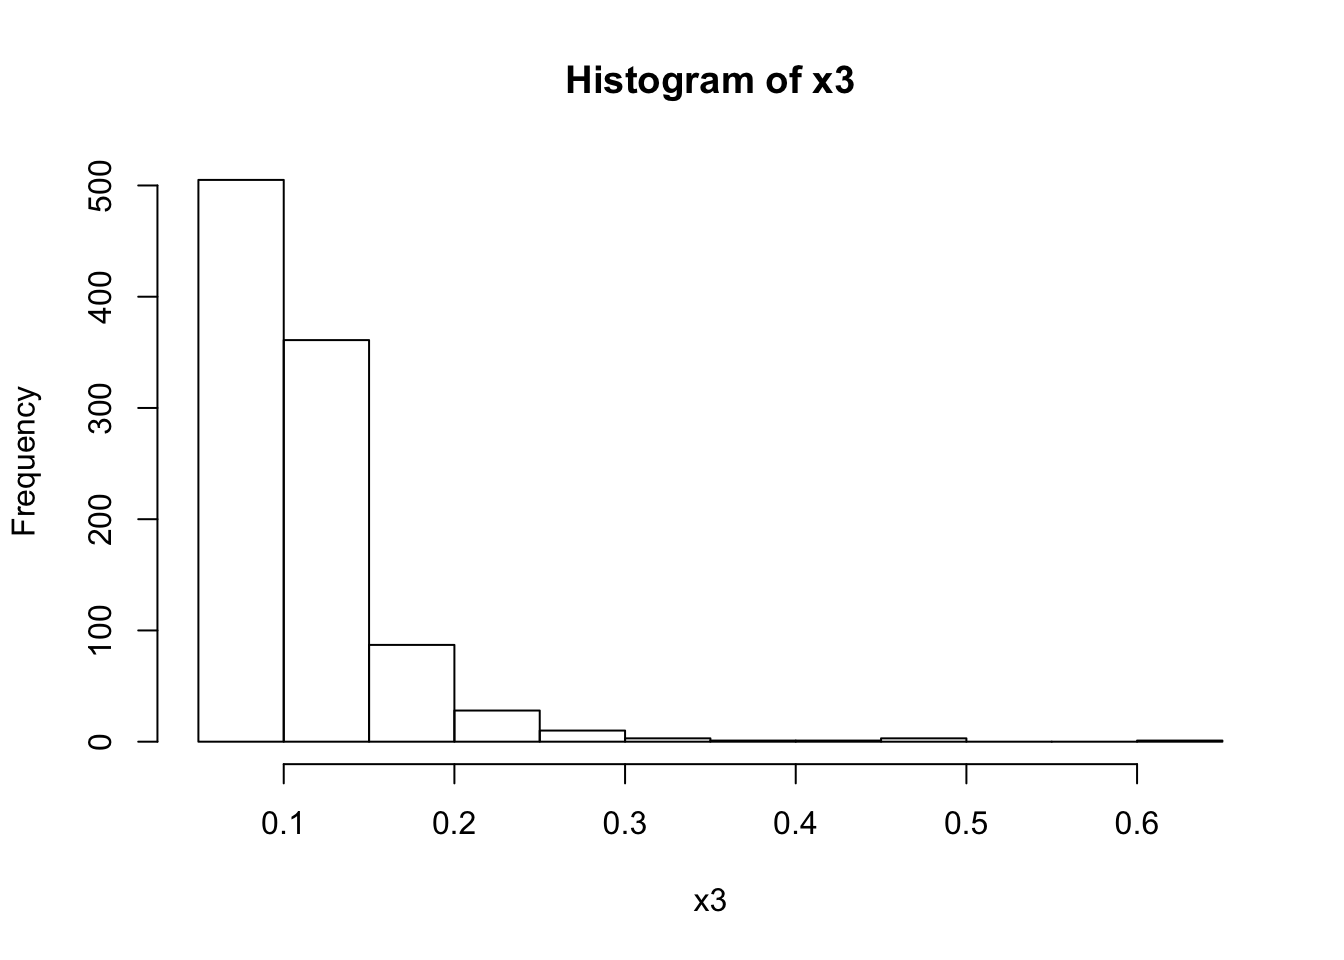
\includegraphics{assignment01-timeseries-psteinke_files/figure-latex/unnamed-chunk-18-1.pdf}
ACF shows not white noise. Shows 3 clear and 5 total outliers outside of
the 0.2 confidence region.

\begin{Shaded}
\begin{Highlighting}[]
\KeywordTok{shapiro.test}\NormalTok{(res.model.ozone.qa) }\CommentTok{# Check normality}
\end{Highlighting}
\end{Shaded}

\begin{verbatim}
## 
##  Shapiro-Wilk normality test
## 
## data:  res.model.ozone.qa
## W = 0.98889, p-value = 0.6493
\end{verbatim}

\hypertarget{hypothesis-for-quadratic}{%
\paragraph{Hypothesis for Quadratic}\label{hypothesis-for-quadratic}}

H0:μΔ=0 HA:μΔ≠0 reject hypothesis because data is not normal The
stochastic component of model 2 is not normally distributed

H0: μt ≠ β0 + β1xt + β2xt2 + εt Ha: μt = β0 + β1xt + β2xt2 + εt

We found that as the p-value was less than 5\% and the null mean
(i.e.~zero) fell within the 95\% confidence interval. As such the null
hypothesis was rejected.

\hypertarget{forecast-for-quadratic-model}{%
\subsection{Forecast for Quadratic
model}\label{forecast-for-quadratic-model}}

\begin{Shaded}
\begin{Highlighting}[]
\KeywordTok{doForecast}\NormalTok{(model.ozone.qa, }\DecValTok{2016}\NormalTok{, }\StringTok{'5 year forecast for quadratic model'}\NormalTok{, }\DataTypeTok{t2=}\NormalTok{T)}
\end{Highlighting}
\end{Shaded}

\begin{verbatim}
##         fit       lwr       upr
## 1 -10.34387 -14.13556 -6.552180
## 2 -10.59469 -14.40282 -6.786548
## 3 -10.84856 -14.67434 -7.022786
## 4 -11.10550 -14.95015 -7.260851
## 5 -11.36550 -15.23030 -7.500701
\end{verbatim}

\includegraphics{assignment01-timeseries-psteinke_files/figure-latex/unnamed-chunk-20-1.pdf}

\hypertarget{harmonic-model}{%
\section{Harmonic Model}\label{harmonic-model}}

\begin{Shaded}
\begin{Highlighting}[]
\NormalTok{har=}\KeywordTok{harmonic}\NormalTok{(ozone.ts,}\FloatTok{0.45}\NormalTok{)}
\NormalTok{model.ozone.har=}\KeywordTok{lm}\NormalTok{(ozone.ts}\OperatorTok{~}\NormalTok{har)}
\KeywordTok{summary}\NormalTok{(model.ozone.har)}
\end{Highlighting}
\end{Shaded}

\begin{verbatim}
## 
## Call:
## lm(formula = ozone.ts ~ har)
## 
## Residuals:
##     Min      1Q  Median      3Q     Max 
## -8.3520 -1.8906  0.4837  2.3643  6.4248 
## 
## Coefficients: (1 not defined because of singularities)
##                  Estimate Std. Error t value Pr(>|t|)    
## (Intercept)    -2.970e+00  4.790e-01  -6.199 1.79e-08 ***
## harcos(2*pi*t)         NA         NA      NA       NA    
## harsin(2*pi*t)  5.462e+11  7.105e+11   0.769    0.444    
## ---
## Signif. codes:  0 '***' 0.001 '**' 0.01 '*' 0.05 '.' 0.1 ' ' 1
## 
## Residual standard error: 3.522 on 88 degrees of freedom
## Multiple R-squared:  0.006672,   Adjusted R-squared:  -0.004616 
## F-statistic: 0.5911 on 1 and 88 DF,  p-value: 0.4441
\end{verbatim}

\begin{itemize}
\tightlist
\item
  p-value = 0.4441 \textgreater{} 0.05, shows the model is insignificant
\item
  Cos = NA
\item
  No seasonality
\item
  Therefore warrants no further investigation
\end{itemize}

\hypertarget{conclusion}{%
\subsection{Conclusion}\label{conclusion}}

\textbf{Task:} Find the best fitting trend model to this dataset

Of our three models, the quadratic trend model was the most successful
fit because it better correlates with the decline towards the end of the
series.

\textbf{Task:} Give predictions of yearly changes for the next 5 years

Utilising the linear and quadratic models, graphs and numeric outputs
with a 5\% variance have been provided.

The data shows an increased rate of decay over time. This does not
appear to be a stationary series, with seasonal pattern and moving
average. Further investigation to find a better fitting model is
warranted.


\end{document}
